\documentclass[8pt, xcolor=table]{beamer}

\usetheme[progressbar=frametitle]{metropolis}
\usepackage{appendixnumberbeamer}
\usepackage{bm}

\usepackage{booktabs}
\usepackage[scale=2]{ccicons}

\usepackage{pgfplots}
\usepgfplotslibrary{dateplot}

\usepackage{xspace}
\newcommand{\themename}{\textbf{\textsc{metropolis}}\xspace}
\usepackage{svg}
\usepackage{xcolor}
\usepackage{amsmath}
\newcommand\norm[1]{\lVert#1\rVert}

\title{Metropolis}
\subtitle{A modern beamer theme}
% \date{\today}
\date{}
\author{Matthias Vogelgesang}
\institute{Center for modern beamer themes}
% \titlegraphic{\hfill\includegraphics[height=1.5cm]{logo.pdf}}

\begin{document}


% \begin{frame}{Table of contents}
%   \setbeamertemplate{section in toc}[sections numbered]
%   \tableofcontents%[hideallsubsections]
% \end{frame}

% \section[Problem Definition \cite{surveyjssp}]{Problem Definition}

\begin{frame}[fragile]{JSSP Definition}
    Several Machines $\bm{M}= \{\bm{M}_1, \bm{M}_2, \ldots, \bm{M}_m\}$\\
    Several Jobs $\bm{J}= \{\bm{J}_1, \bm{J}_2, \ldots,\bm{J}_i,\ldots, \bm{J}_n\}$ \\
    each job $\bm{J}_i$ contains several operations\\
    $\bm{O_i}= \{\bm{O}_{i1}, \bm{O}_{i2},\ldots, \bm{O}_{in}\}$ which need to be processed in a predefined technological sequence\\
    Each operation is assigned a machine in $\bm{M}$ to be processed with a given processing time $p_{ij}$
\end{frame}

\begin{frame}[fragile]{Subtypes of JSSP}
    \begin{figure}[H]
      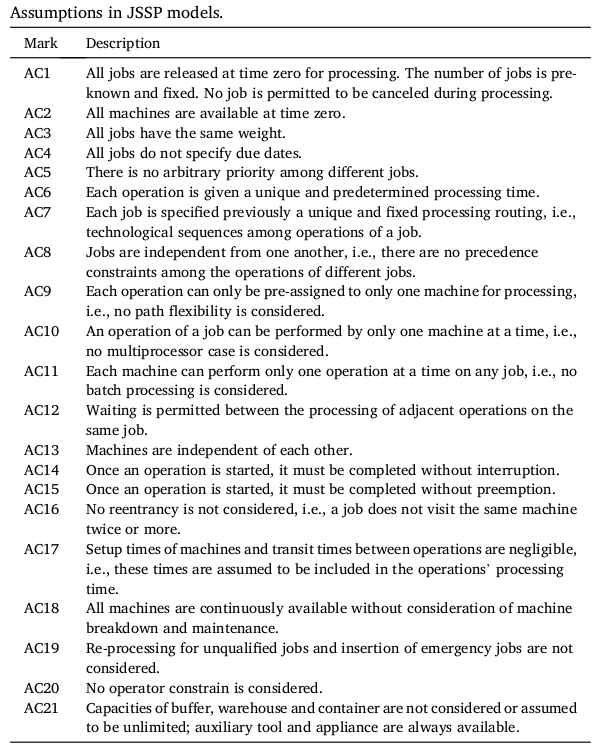
\includegraphics[width=0.62\textwidth]{img/subtypes.png}
    \end{figure}
\end{frame}

\begin{frame}[fragile]{Objectives}
  \begin{minipage}[t]{0.55\textwidth}
    \begin{figure}[H]
      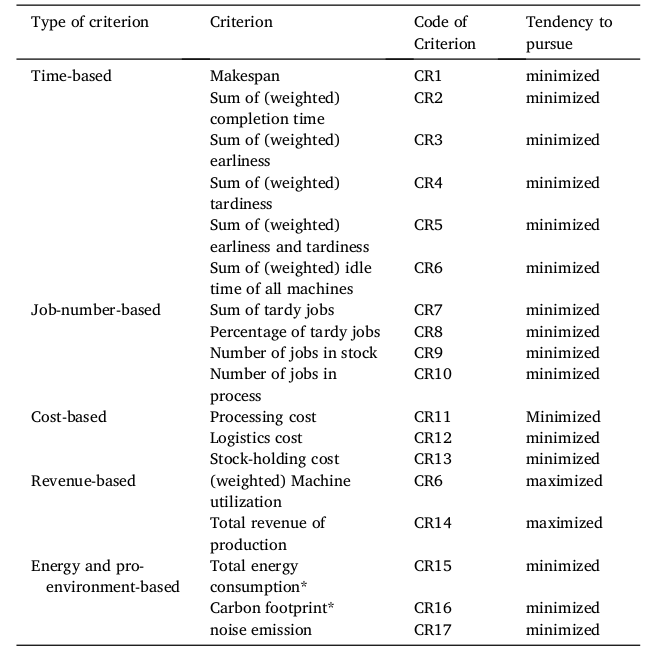
\includegraphics[width=\textwidth]{img/objective.png}
    \end{figure}
  \end{minipage}
  \begin{minipage}[t]{0.4\textwidth}
    \begin{figure}[H]
      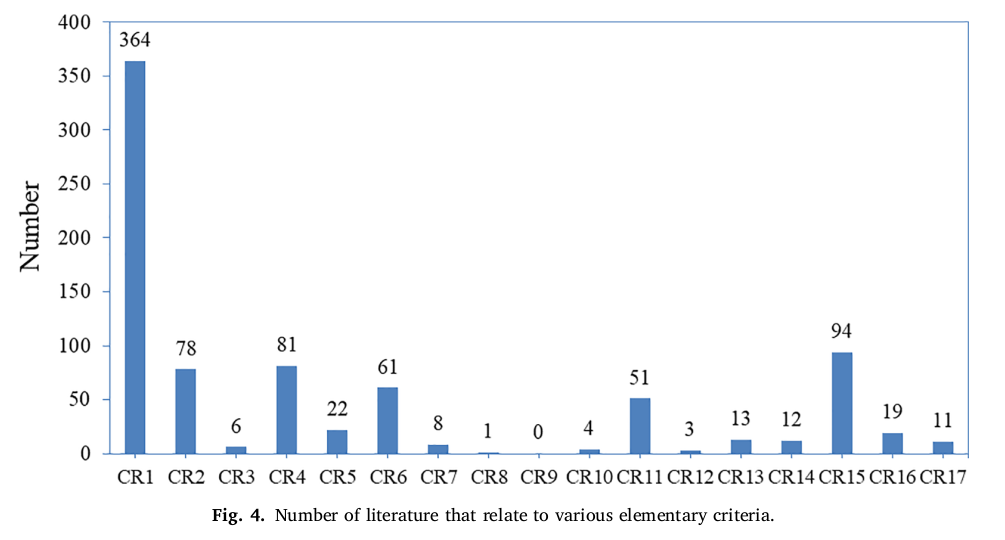
\includegraphics[width=\textwidth]{img/Objective_distr.png}
    \end{figure}
  \end{minipage}
\end{frame}

\begin{frame}[fragile]{Entities Values}
  \begin{minipage}[t]{0.4\textwidth}
    \begin{figure}[H]
      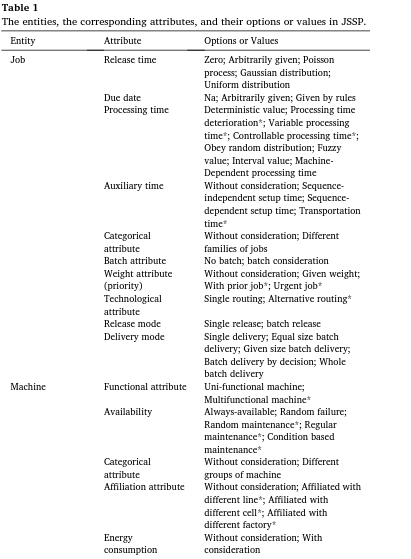
\includegraphics[width=\textwidth]{img/entities1.png}
    \end{figure}
  \end{minipage}
  \begin{minipage}[t]{0.5\textwidth}
    \begin{figure}[H]
      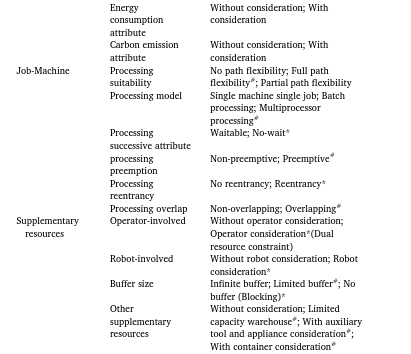
\includegraphics[width=\textwidth]{img/entities2.png}
    \end{figure}
  \end{minipage}
\end{frame}


\begin{frame}[fragile]{Most Famous Subtypes of JSSP}
  \begin{itemize}
    \item \textbf{Classical JSSP}: All assumptions are involved
    \item \textbf{Dynamic JSSP}: Relax AC1, AC4, AC6 or AC19. Dynamism in the jobs
    \item \textbf{Flexible JSSP}: Relax AC7, AC9. Flexibility in operation ordering or more machine available for an operation
  \end{itemize}
\end{frame}

\begin{frame}[fragile]{Dynamical JSSP}
  \begin{itemize}
    \item \textbf{AC1} All jobs are released at time zero for processing. The number of jobs is pre-
    known and fixed. No job is permitted to be canceled during processing.
    \item \textbf{AC4} All jobs do not specify due dates.
    \item \textbf{AC6} Each operation is given a unique and predetermined processing time.
  \end{itemize}
\end{frame}

\begin{frame}[fragile]{Flexible JSSP}
  \begin{itemize}
    \item \textbf{AC7} Each job is specified previously a unique and fixed processing routing, i.e.,
    technological sequences among operations of a job.
    \item \textbf{AC9} Each operation can only be pre-assigned to only one machine for processing,
    i.e., no path flexibility is considered.
  \end{itemize}
\end{frame}

\begin{frame}[fragile]{Most Used Algorithms}
  \begin{itemize}
    \item Mixed Integer Programming
    \item Meta Heuristics (aka Evolutionary)
    \begin{itemize}
      \item Ant Colony 
      \item Hill Climbing
      \item Stochastic Local Search
      \item Genetic Algorithms
    \end{itemize}
  \end{itemize}
\end{frame}


\begin{frame}[fragile]{JSSP considering robot/AGV}
  Robots and AGVs are widely used in the real-life manufacturing
  systems to improve productivity, reduce cost and achieve better quality.
  It is more computationally difficult than the JSP presenting
  two additional difficulties caused by \alert{a set of jobs to be processed
  on a set of alternative machines and to be transported between
  them by many robots.}
\end{frame}


\begin{frame}[allowframebreaks]{References}
  \bibliography{demo}
  \bibliographystyle{abbrv}
\end{frame}

\end{document}
